\documentclass[a4paper,12pt]{article}
\usepackage[utf8]{inputenc}  % Soporte para caracteres UTF-8
\usepackage{amsmath, amssymb} % Paquetes para matemáticas
\usepackage{graphicx} % Para incluir imágenes
\usepackage{hyperref} % Para enlaces y referencias cruzadas
\usepackage{booktabs}
\usepackage{geometry}
\usepackage{float}
\usepackage{array}
\usepackage{geometry} % Para ajustar márgenes
\geometry{margin=1in} % Márgenes de 1 pulgada

\title{Time Series Analysis and LSTM-based Models Comparission Using Solar Photovoltaic Electricity
Generation at CIC-IPN in North of Mexico City}
\author{P.J Escamilla Ambrosio\\
        \textit{Centro de Investigación en Computación}\\
        \and
        R. Alcaraz Fraga\\
        \textit{Escuela Superior de Física y Matemáticas}\\
        }
\date{\today}

\begin{document}

\maketitle

\begin{abstract}
This paper presents a comprehensive comparison between classical time series prediction models, such as ARIMA and Holt-Winters, and more advanced approaches based on neural networks, specifically Long Short-Term Memory (LSTM). Multiple datasets from different domains are evaluated with the aim of determining which model offers better performance in terms of accuracy and generalization ability. The results show that, while traditional models offer interpretability and are effective in certain situations, LSTM-based models outperform them in complex problems with long-term dependencies. Furthermore, the advantages and disadvantages of each approach are discussed based on computational requirements and the amount of data needed for effective training. This study provides a practical guide for selecting the appropriate model depending on the context and the available data.
\end{abstract}

\section{Introduction}
Solar photovoltaic (SPV) power generation is inherently dependent on various environmental factors, such as sunlight intensity, temperature, and weather conditions, which can vary significantly over time. Accurate forecasting of SPV energy output is essential for integrating this renewable energy source into existing power grids and ensuring its stability and reliability. Traditional time series models, such as ARIMA and Holt-Winters, have been widely used for forecasting in various domains due to their simplicity and interpretability. However, these models often struggle to capture complex, nonlinear patterns present in renewable energy data, especially when dealing with long-term dependencies.

In recent years, more advanced methods based on neural networks, particularly Long Short-Term Memory (LSTM) networks, have gained attention for their ability to model sequential data with intricate patterns. LSTM networks, a type of recurrent neural network (RNN), are specifically designed to handle long-term dependencies, making them suitable for time series prediction tasks with variable dynamics and nonlinearity.

This study aims to compare the performance of traditional time series models and LSTM networks in forecasting SPV energy output. By evaluating these models on real-world datasets, we seek to identify the advantages and limitations of each approach, providing insights into their applicability for energy forecasting in renewable energy systems.

\section{Related Work}

\section{Solar Photovoltaic Electricity Generation Prediction}
In this section, the solar photovoltaic electricity generation plant installed at CIC-IPN
is described, along with the electricity generation data that have been obtained since the
activation of the SPV plant. Afterwards, time series forecasting of the collected data is per-
formed and the results obtained are presented.

\subsection{Solar Photovoltaic Plant}
The data used were obtained from the solar photovoltaic (SPV) electricity generation
plant installed at CIC-IPN [6], located in north Mexico City, 19° 30' 11.1" North-lati-
tude, 99° 08' 52.1" West-longitude at 2,243 m altitude, see Fig.1. The SPV plant has
186 solar panels (Canadian Solar CS3U), connected to three inverters (each Fronius
Symo, 22.7 kW) with a maximum power capacity of 66.96 kW.

\subsection{SPV Data}
Data collected from this SPV plant includes several parameters, but the ones used in
this research include photovoltaic production (Wh), irradiance (W/m2), ambient tem-
perature (°C), panel temperature (°C) and variables related to the electric current of the sensors contained on the SPV panels (A). This data corresponds to 1101 days ranging from 25-10-2019 to 31-12-2023.

\section{Time Series Analysis}

Time series analysis involves examining data points collected or recorded at specific time intervals to identify patterns, trends, and relationships within the data. This type of analysis is crucial in various fields, including economics, finance, weather forecasting, and energy production, as it allows for modeling and predicting future outcomes based on historical data.

A fundamental aspect of time series analysis is understanding the components that constitute a time series. These components typically include:

\begin{itemize}
    \item \textbf{Trend}: The long-term movement or direction in the data, indicating whether the series is increasing, decreasing, or remaining constant over time.
    \item \textbf{Seasonality}: Regular, periodic fluctuations that occur within the series, often corresponding to specific times of the year, month, or week.
    \item \textbf{Cyclic Patterns}: Non-seasonal, long-term oscillations that can be attributed to economic cycles, technological advancements, or other systemic factors.
    \item \textbf{Random Variation}: The irregular, unpredictable fluctuations that do not follow a pattern and are often considered as noise.
\end{itemize}

Identifying and analyzing these components help in building accurate models for forecasting and understanding the underlying processes generating the data. Techniques such as decomposition methods, autocorrelation analysis, and spectral analysis are commonly employed to dissect and interpret time series data.

In the context of this study, time series analysis is pivotal for understanding the temporal patterns in solar photovoltaic (SPV) energy production. By analyzing the time series data of SPV output, we can develop models to predict future energy generation, which is essential for efficient energy planning and grid integration.

\subsection{SARIMAX}

Time series analysis plays a crucial role in various fields such as economics, finance, and environmental studies. Among the many models developed for time series forecasting, the Seasonal Autoregressive Integrated Moving Average with eXogenous inputs (SARIMAX) model stands out for its flexibility and effectiveness in capturing different patterns within the data.

The SARIMAX model extends the Autoregressive Integrated Moving Average (ARIMA) model by incorporating seasonal components and external regressors. The general form of the SARIMAX model can be expressed as:

\begin{equation}
Y_t = \phi_1 Y_{t-1} + \phi_2 Y_{t-2} + \ldots + \phi_p Y_{t-p} + \theta_1 \varepsilon_{t-1} + \theta_2 \varepsilon_{t-2} + \ldots + \theta_q \varepsilon_{t-q} + \varepsilon_t
\end{equation}

where:
\begin{itemize}
    \item \(Y_t\) is the value of the time series at time \(t\),
    \item \(\phi_i\) are the autoregressive parameters,
    \item \(\theta_i\) are the moving average parameters,
    \item \(\varepsilon_t\) is a white noise error term,
    \item \(p\) is the order of the autoregressive part,
    \item \(q\) is the order of the moving average part.
\end{itemize}
 
The seasonal aspect of the model is incorporated through the parameters \(P\), \(D\), and \(Q\), which represent the seasonal autoregressive order, the seasonal differencing order, and the seasonal moving average order, respectively. The SARIMAX model is thus denoted as:

\begin{equation}
SARIMAX(p, d, q)(P, D, Q)_s
\end{equation}

where \(s\) denotes the length of the seasonal cycle. 

The ability of the SARIMAX model to accommodate both seasonal patterns and external variables makes it particularly powerful for forecasting applications. 

\section{Deep Neural Networks}

Neural networks have emerged as a powerful class of models for solving complex problems in various domains, including computer vision, natural language processing, and time series forecasting. Inspired by the biological neural networks in the human brain, artificial neural networks (ANNs) consist of interconnected nodes, or neurons, that process information in a layered architecture.

A typical neural network can be mathematically represented as follows:

\begin{equation}
Y = f(W \cdot X + b)
\end{equation}

where:
\begin{itemize}
    \item \(Y\) is the output vector,
    \item \(f\) is the activation function (e.g., sigmoid, ReLU),
    \item \(W\) is the weight matrix,
    \item \(X\) is the input vector,
    \item \(b\) is the bias vector.
\end{itemize}

The activation function introduces non-linearity into the model, enabling it to learn complex patterns. Common choices for activation functions include:

\begin{itemize}
    \item Sigmoid: \(f(x) = \frac{1}{1 + e^{-x}}\)
    \item Hyperbolic Tangent: \(f(x) = \tanh(x)\)
    \item Rectified Linear Unit (ReLU): \(f(x) = \max(0, x)\)
\end{itemize}

The training process of a neural network involves optimizing the weights and biases to minimize the loss function, which quantifies the difference between the predicted outputs and the actual targets. A popular choice for the loss function in regression tasks is the mean squared error (MSE):

\begin{equation}
L = \frac{1}{n} \sum_{i=1}^{n} (y_i - \hat{y}_i)^2
\end{equation}

where \(y_i\) is the actual output and \(\hat{y}_i\) is the predicted output.

Recent advancements in deep learning, particularly with the introduction of deep neural networks (DNNs), have further enhanced the capability of neural networks to model high-dimensional data.

\subsection{LSTM}

Long Short-Term Memory (LSTM) networks are a specialized type of recurrent neural network (RNN) designed to effectively capture long-range dependencies in sequential data. Traditional RNNs suffer from issues such as vanishing and exploding gradients, which make it difficult for them to learn long-term patterns. LSTMs address this limitation through their unique architecture, enabling them to retain information over extended periods.

The LSTM unit consists of a cell state, along with three gates: the input gate, the forget gate, and the output gate. The cell state serves as the long-term memory, while the gates control the flow of information into and out of the cell. Mathematically, the operations of an LSTM cell at time step \(t\) can be described as follows:

1. Forget Gate:
\begin{equation}
f_t = \sigma(W_f \cdot [h_{t-1}, x_t] + b_f)
\end{equation}
where \(f_t\) is the forget gate's output, \(W_f\) is the weight matrix for the forget gate, \(h_{t-1}\) is the hidden state from the previous time step, \(x_t\) is the current input, and \(b_f\) is the bias term. The sigmoid activation function \(\sigma\) outputs values between 0 and 1, determining how much of the previous cell state to retain.

2. Input Gate:
\begin{equation}
i_t = \sigma(W_i \cdot [h_{t-1}, x_t] + b_i)
\end{equation}
\begin{equation}
\tilde{C}_t = \tanh(W_C \cdot [h_{t-1}, x_t] + b_C)
\end{equation}
The input gate \(i_t\) decides how much of the new information to incorporate, and \(\tilde{C}_t\) is a candidate value that may be added to the cell state, with \(W_i\) and \(W_C\) being their respective weight matrices, and \(b_i\) and \(b_C\) the corresponding bias terms.

3. Cell State Update:
\begin{equation}
C_t = f_t \cdot C_{t-1} + i_t \cdot \tilde{C}_t
\end{equation}
This equation updates the cell state \(C_t\) by combining the retained information from the previous cell state and the new candidate values.

4. Output Gate:
\begin{equation}
o_t = \sigma(W_o \cdot [h_{t-1}, x_t] + b_o)
\end{equation}
\begin{equation}
h_t = o_t \cdot \tanh(C_t)
\end{equation}
The output gate \(o_t\) determines the next hidden state \(h_t\), which is influenced by the current cell state \(C_t\). Here, \(W_o\) is the weight matrix for the output gate, and \(b_o\) is the bias term.

The architecture of LSTM networks allows them to effectively learn from sequences where contextual information is spread over long intervals, making them particularly suitable for applications in natural language processing, time series forecasting, and more.

\section{SPV Data Processing}
The available data on SPV generation contains several details that need to be addressed before using it on any model. This section contains the taken steps to process the data in order for it to be ready to be used.

\subsection{Complete Days}

The SPV data is measured each 5 minutes, in order to keep consistence, only days with "complete" data points are used, therefore, only days with 288 data points are selected, since measures each 5 minutes per day results in 288 measures a day. Performing this selection, the number of rows reduces from 333,775 and 1176 days to 317,088 and 1101 days.

\subsection{NaN Values for SPV Generation}
Values of SPV generation present some NaN. This is problematic as this variable is our target, therefore this problem needs to be addressed. It is important to note that there are intervals in which this production is 0, these intervals are composed of hours in which there tends to be no solar light. If a NaN is found in this interval, it is replaced by 0, and if it is outside of this interval, it is replaced with the mean of the SPV generation value in \(t-1\) and \(t+1\). 

It is worth noticing that some days have no NaN values at all, so this days are used to build this interval. To find the interval an agrupation by hour was made and then the data was filtered by SPV generation values of 0, the interval contains the hours in which the count of SPV values of 0 is greater than 3, in order to avoid data measurement errors (hours which are supposed to have values different from 0 containing values of 0 due to sensors errors).

By analyzing the data, the interval was found to be from 00:00 to 07:40 and from 17:35 to 23:55.

\subsection{NaN Values for Relevant Variables}
While it is true that for SARIMAX no further information is needed this is not the case for LSTM, and so relevant variables are selected to train this model. The way in which this variables were chosen is by their correlation with SPV generation. A correlation greater than 0.7 is going to be taken as relevant. The data starts off with 58 columns, once the correlation analysis was made this columns were reduced to 35. Following are the obtained correlations:

\begin{table}[H]
\centering
\begin{tabular}{ll}
\toprule
\textbf{Column} & \textbf{Correlation} \\
\midrule
Potencia reactiva | Symo 22.7-3 480 (Norte) & -0.85714 \\
Potencia reactiva | Symo 22.7-3 480 (Sur) & -0.79278 \\
Temperatura de módulo | Sensor Card / Box (1) & 0.908048 \\
Corriente CC MPP1 | Symo 22.7-3 480 (1) & 0.964973 \\
Energía MPP1 | Symo 22.7-3 480 (1) & 0.968674 \\
Irradiación | Sensor Card / Box (1) & 0.98559 \\
Corriente CC MPP2 | Symo 22.7-3 480 (1) & 0.987772 \\
Corriente CA L2 | Symo 22.7-3 480 (1) & 0.990479 \\
Rendimiento específico | Symo 22.7-3 480 (1) & 0.990489 \\
Energía | Symo 22.7-3 480 (1) & 0.990489 \\
Potencia aparente | Symo 22.7-3 480 (1) & 0.990489 \\
Corriente CA L1 | Symo 22.7-3 480 (1) & 0.990547 \\
Corriente CA L3 | Symo 22.7-3 480 (1) & 0.990605 \\
Energía MPP2 | Symo 22.7-3 480 (1) & 0.991791 \\
Corriente CC MPP2 | Symo 22.7-3 480 (Sur) & 0.996317 \\
Corriente CA L1 | Symo 22.7-3 480 (Sur) & 0.99654 \\
Corriente CA L3 | Symo 22.7-3 480 (Sur) & 0.99655 \\
Corriente CA L2 | Symo 22.7-3 480 (Sur) & 0.996572 \\
Corriente CC MPP1 | Symo 22.7-3 480 (Sur) & 0.996627 \\
Energía MPP2 | Symo 22.7-3 480 (Sur) & 0.997757 \\
Corriente CC MPP1 | Symo 22.7-3 480 (Norte) & 0.997762 \\
Corriente CC MPP2 | Symo 22.7-3 480 (Norte) & 0.99782 \\
Potencia aparente | Symo 22.7-3 480 (Sur) & 0.997929 \\
Energía | Symo 22.7-3 480 (Sur) & 0.997982 \\
Rendimiento específico | Symo 22.7-3 480 (Sur) & 0.997982 \\
Energía MPP1 | Symo 22.7-3 480 (Sur) & 0.998017 \\
Corriente CA L1 | Symo 22.7-3 480 (Norte) & 0.998059 \\
Corriente CA L3 | Symo 22.7-3 480 (Norte) & 0.998069 \\
Corriente CA L2 | Symo 22.7-3 480 (Norte) & 0.998071 \\
Energía MPP1 | Symo 22.7-3 480 (Norte) & 0.998143 \\
Potencia aparente | Symo 22.7-3 480 (Norte) & 0.998404 \\
Rendimiento específico | Symo 22.7-3 480 (Norte) & 0.998456 \\
Energía | Symo 22.7-3 480 (Norte) & 0.998456 \\
Energía MPP2 | Symo 22.7-3 480 (Norte) & 0.998593 \\
Producción fotovoltaica & 1.0 \\
\bottomrule
\end{tabular}
\caption{Correlations between columns}
\label{tab:correlations}
\end{table}

This columns also contain NaN values in the following proportions
\begin{table}[H] % Usar el modificador H
\centering
\begin{tabular}{ll}
\toprule
\textbf{Column} & \textbf{NaN Percentage} \\
\midrule
Producción fotovoltaica & 0.000000 \\
Corriente CC MPP1 | Symo 22.7-3 480 (1) & 0.065975 \\
Energía MPP1 | Symo 22.7-3 480 (1) & 0.065975 \\
Corriente CC MPP2 | Symo 22.7-3 480 (1) & 0.065975 \\
Corriente CA L2 | Symo 22.7-3 480 (1) & 0.065975 \\
Rendimiento específico | Symo 22.7-3 480 (1) & 0.065975 \\
Energía | Symo 22.7-3 480 (1) & 0.065975 \\
Potencia aparente | Symo 22.7-3 480 (1) & 0.065975 \\
Corriente CA L1 | Symo 22.7-3 480 (1) & 0.065975 \\
Corriente CA L3 | Symo 22.7-3 480 (1) & 0.065975 \\
Energía MPP2 | Symo 22.7-3 480 (1) & 0.065975 \\
Temperatura de módulo | Sensor Card / Box (1) & 0.459484 \\
Irradiación | Sensor Card / Box (1) & 0.459484 \\
Corriente CC MPP1 | Symo 22.7-3 480 (Sur) & 0.460598 \\
Corriente CA L3 | Symo 22.7-3 480 (Sur) & 0.460598 \\
Corriente CA L2 | Symo 22.7-3 480 (Sur) & 0.460598 \\
Corriente CC MPP2 | Symo 22.7-3 480 (Sur) & 0.460598 \\
Corriente CA L1 | Symo 22.7-3 480 (Sur) & 0.460598 \\
Energía | Symo 22.7-3 480 (Norte) & 0.461847 \\
Rendimiento específico | Symo 22.7-3 480 (Norte) & 0.461847 \\
Potencia aparente | Symo 22.7-3 480 (Norte) & 0.461847 \\
Energía MPP1 | Symo 22.7-3 480 (Norte) & 0.461847 \\
Corriente CA L2 | Symo 22.7-3 480 (Norte) & 0.461847 \\
Corriente CA L3 | Symo 22.7-3 480 (Norte) & 0.461847 \\
Corriente CA L1 | Symo 22.7-3 480 (Norte) & 0.461847 \\
Potencia reactiva | Symo 22.7-3 480 (Norte) & 0.461847 \\
Corriente CC MPP2 | Symo 22.7-3 480 (Norte) & 0.461847 \\
Corriente CC MPP1 | Symo 22.7-3 480 (Norte) & 0.461847 \\
Energía MPP2 | Symo 22.7-3 480 (Norte) & 0.461847 \\
Energía | Symo 22.7-3 480 (Sur) & 0.463427 \\
Potencia aparente | Symo 22.7-3 480 (Sur) & 0.463427 \\
Energía MPP2 | Symo 22.7-3 480 (Sur) & 0.463427 \\
Potencia reactiva | Symo 22.7-3 480 (Sur) & 0.463427 \\
Rendimiento específico | Symo 22.7-3 480 (Sur) & 0.463427 \\
Energía MPP1 | Symo 22.7-3 480 (Sur) & 0.463427 \\
\bottomrule
\end{tabular}
\caption{NaN percentage for relevant columns}
\label{tab:nan_percentages}
\end{table}

This NaN values are imputed using a forward-fill algorithm, which imputes NaN values with the last (non NaN value) observed in the data. For this to function, the first NaN values of each day needs to be set to 0. Descriptive statistics of some columns can be observed in the following table

\begin{table}[H]
    \centering
    \begin{tabular}{l p{2.5cm} p{2.5cm} p{2.5cm} p{2.5cm} p{2.5cm}}
        \toprule
        & \textbf{Potencia reactiva | Symo 22.7-3 480 (Norte)} & \textbf{Potencia reactiva | Symo 22.7-3 480 (Sur)} & \textbf{Temperatura de módulo | Sensor Card / Box (1)} & \textbf{Irradiación | Sensor Card / Box (1)} & \textbf{Energía | Symo 22.7-3 480 (1)} \\
        \midrule
        count & 317088.000000 & 317088.000000 & 317088.000000 & 317088.000000 & 317088.000000 \\
        mean & -7.953227 & -3.132833 & 25.812104 & 199.773331 & 204.156066 \\
        std & 36.524708 & 40.943096 & 12.551188 & 289.796911 & 302.065523 \\
        min & -146.400000 & -151.710000 & -1.000000 & -1.000000 & 0.000000 \\
        25\% & 0.000000 & 0.000000 & 17.000000 & 0.000000 & 0.000000 \\
        50\% & 0.000000 & 0.000000 & 21.000000 & 0.000000 & 0.000000 \\
        75\% & 7.530000 & 28.270000 & 34.000000 & 367.000000 & 376.883570 \\
        max & 62.240000 & 75.130000 & 63.000000 & 1255.000000 & 1634.775880 \\
        \bottomrule
    \end{tabular}
   \caption{Descriptive statistics for some relevant columns}
\end{table}

\subsection{Results of Processing}
At the end of the processing, the data is ready to be used in the SARIMAX and LSTM models. As a side note, interesting things came up from this process. The first thing that can be noticed is that the data is fairly distributed between months as it can be seen in the following graph.

\begin{figure}[H] % [H] coloca la imagen exactamente en el lugar donde aparece en el texto
    \centering % Centra la imagen
    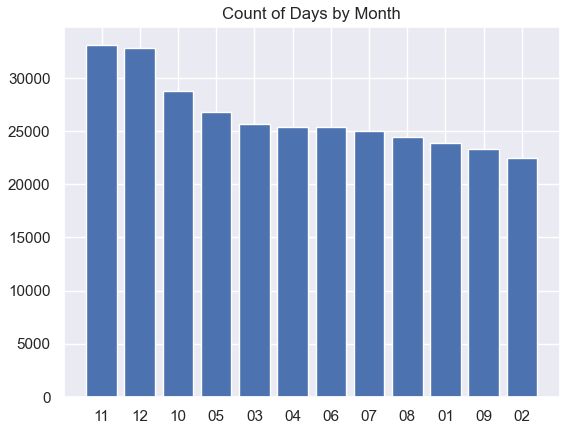
\includegraphics[height=0.40\textwidth]{conteo.png} % Ajusta el ancho de la imagen
    \caption{Number of days in each season of the year} % Leyenda de la imagen
    \label{fig:etiqueta_imagen} % Etiqueta para referirse a la imagen en el texto
\end{figure}

\begin{figure}[H] % [H] coloca la imagen exactamente en el lugar donde aparece en el texto
    \centering % Centra la imagen
    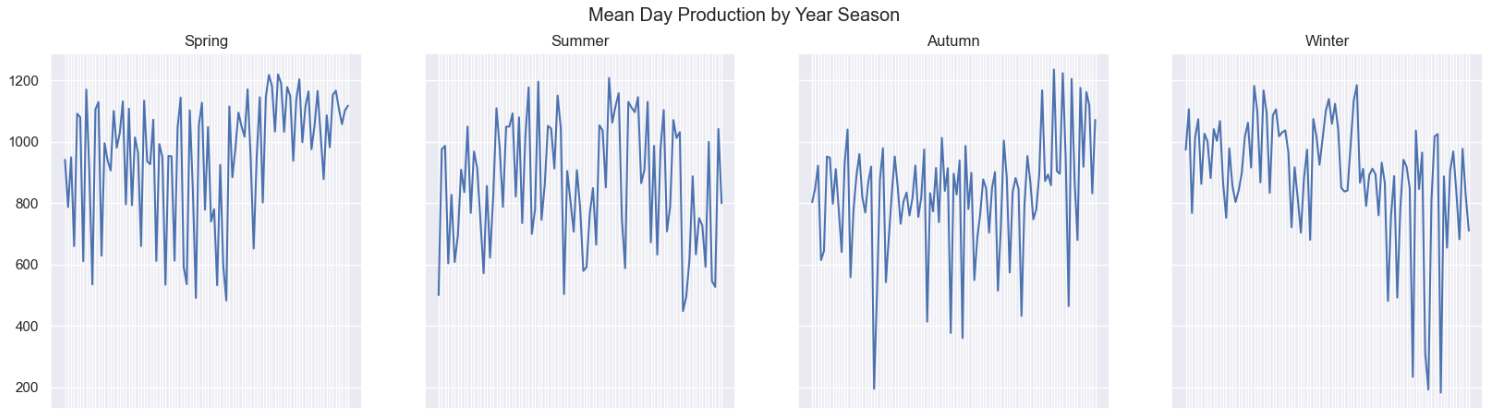
\includegraphics[width=1\textwidth]{temporada.png} % Ajusta el ancho de la imagen
    \caption{Mean production by day and season of the year} % Leyenda de la imagen
    \label{fig:etiqueta_imagen} % Etiqueta para referirse a la imagen en el texto
\end{figure}

\section{Time Series Analysis}
As the data is ready to be used in models, this section takes on the performed time series analysis. First of all, the first ten days of the data can be seen on the following graph

\begin{figure}[H] % [H] coloca la imagen exactamente en el lugar donde aparece en el texto
    \centering % Centra la imagen
    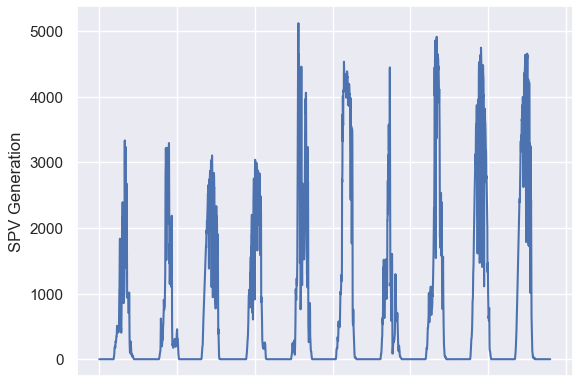
\includegraphics[height=0.35\textwidth]{tendays.png} % Ajusta el ancho de la imagen
    \caption{First ten days of SPV generation} % Leyenda de la imagen
    \label{fig:etiqueta_imagen} % Etiqueta para referirse a la imagen en el texto
\end{figure} 

Performing a augmented Dickey-Fuller test shows the following results

\begin{table}[H]
    \centering
    \begin{tabular}{>{\raggedright\arraybackslash}p{5cm} p{5cm}} % Ajusta el ancho de las columnas según sea necesario
        \toprule
        \textbf{Values} & \textbf{Metric} \\
        \midrule
        -57.682661 & Test Statistics \\
        0.000000 & p-value \\
        76.000000 & No. of lags used \\
        158927.000000 & Number of observations used \\
        -3.430391 & Critical value (1\%) \\
        -2.861558 & Critical value (5\%) \\
        -2.566780 & Critical value (10\%) \\
        \bottomrule
    \end{tabular}
    \caption{Dickey-Fuller test results}
\end{table}

From this values we can observe that the time series is stationary since the p-value is not greater than 5\%, this can also be observed in the following time series decomposition

\begin{figure}[H] % [H] coloca la imagen exactamente en el lugar donde aparece en el texto
    \centering % Centra la imagen
    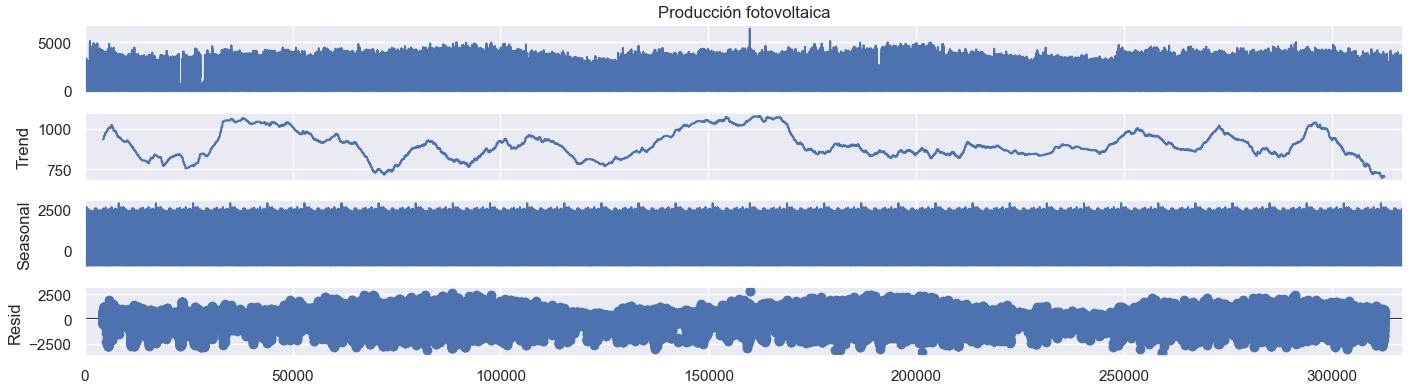
\includegraphics[width=1\textwidth]{decomposition.png} % Ajusta el ancho de la imagen
    \caption{Time series decomposition of the SPV generation time series} % Leyenda de la imagen
    \label{fig:etiqueta_imagen} % Etiqueta para referirse a la imagen en el texto
\end{figure} 

The trend does not increase or decrease.

\subsection{Time Series Forecasting}
The forecasting was realized following the next train/test split.

\begin{figure}[H] % [H] coloca la imagen exactamente en el lugar donde aparece en el texto
    \centering % Centra la imagen
    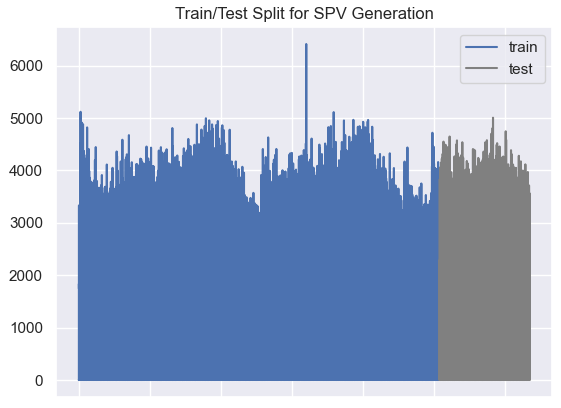
\includegraphics[height=0.35\textwidth]{traintest.png} % Ajusta el ancho de la imagen
    \caption{Time series decomposition of the SPV generation time series} % Leyenda de la imagen
    \label{fig:etiqueta_imagen} % Etiqueta para referirse a la imagen en el texto
\end{figure} 

After fitting the ARIMA model the following results can be observed.

\begin{figure}[H] % [H] coloca la imagen exactamente en el lugar donde aparece en el texto
    \centering % Centra la imagen
    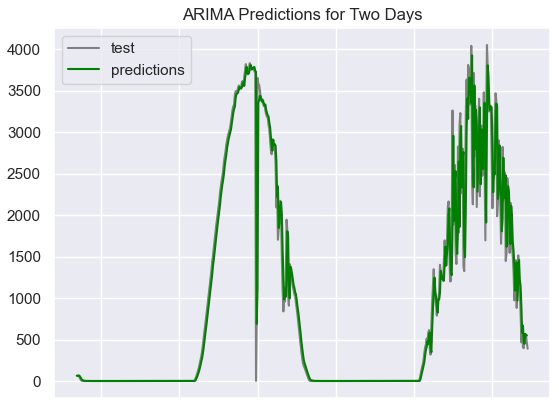
\includegraphics[height=0.35\textwidth]{ARIMA.png} % Ajusta el ancho de la imagen
    \caption{ARIMA Predictions of Two Days} % Leyenda de la imagen
    \label{fig:etiqueta_imagen} % Etiqueta para referirse a la imagen en el texto
\end{figure} 

By comparing the test set and the ARIMA predictions a MSE of 143068.8 can be found.

\section{LSTM}
Training the LSTM model follows the train/test. The LSTM model is configured with RELU as activation function, the model was trained for 100 epochs and a batch size of 128. The results can be seen on the following graph

\begin{figure}[H] % [H] coloca la imagen exactamente en el lugar donde aparece en el texto
    \centering % Centra la imagen
    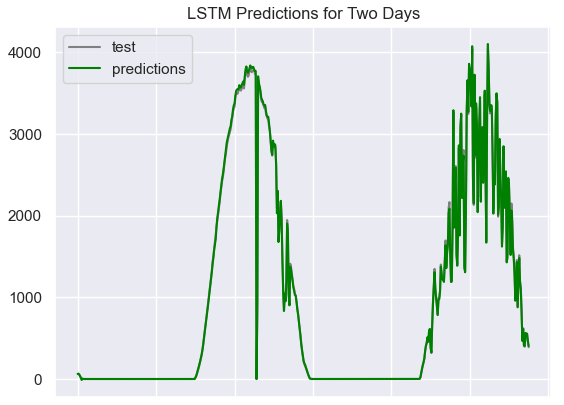
\includegraphics[height=0.35\textwidth]{LSTM.png} % Ajusta el ancho de la imagen
    \caption{LSTM Predictions of Two Days} % Leyenda de la imagen
    \label{fig:etiqueta_imagen} % Etiqueta para referirse a la imagen en el texto
\end{figure} 

By comparing the test set and the ARIMA predictions a MSE of 571.8 can be found.

\begin{thebibliography}{99}
\bibitem{referencia1}
Box, G. E. P., Jenkins, G. M., \& Reinsel, G. C. (2015). Time Series Analysis: Forecasting and Control. Wiley.

\bibitem{referencia2}
Hyndman, R. J., \& Athanasopoulos, G. (2018). Forecasting: Principles and Practice. OTexts.

\bibitem{referencia3}
Goodfellow, I., Bengio, Y., \& Courville, A. (2016). Deep Learning. MIT Press.

\end{thebibliography}

\end{document}
